% ============================================================
%  appendix_benchmark_tables.tex
%  Appendix: Detailed Benchmark Tables (moved out of Chapter 6)
% ============================================================
% !TEX root = Thesis.tex

\chapter{Detailed Benchmark Tables}
\label{app:benchmark-tables}

This appendix collects the detailed cross-system benchmark tables
referenced in Chapter~\ref{chap:evaluation}.  They are reproduced here
for completeness and reproducibility, while the summary tables and the
key findings stay in the chapter body.  Unless a table says otherwise,
the figures come from the Amazon UK Products benchmark under the
cross-system protocol set out below.

\section{Measurement Provenance and Reproducibility}
\label{app:provenance}

\paragraph{Engine under test.}
Every engine figure in this thesis comes from one build of the
implementation, left unmodified across all four campaigns.  Its
regression suite collects and passes \textbf{702} tests.

\paragraph{Benchmark protocols.}
Four campaigns, each with a fixed protocol:

\begin{itemize}
  \item \textbf{Cross-system matrix} --- 1 CPU, 32\,GB, 5 warm-up and
    20 measured runs, 1.5$\times$ IQR filtering, ordered input,
    warm cache; 5 pattern families $\times$ 6 sizes (100\,K--2\,222\,742)
    $=$ 30 engine cells.
  \item \textbf{Stress} --- dedicated control group, 1 CPU, 58\,GB,
    2 warm-up and 5 measured runs, 600\,s per-query budget, restart per
    size; 5 families $\times$ 7 sizes (5\,M--227\,899\,533) $=$ 35 cells.
  \item \textbf{Ordering} --- as the matrix, with each input's physical
    row order shuffled deterministically
    (\texttt{random\_state}~$=1234+\text{size}$), forcing a genuine sort.
  \item \textbf{State-dependent worst case} --- as the matrix, with
    \texttt{B AS category='B' AND price > AVG(A.price)}, ordered input.
\end{itemize}

Memory is sampled from the control group's \texttt{memory.current} every
50\,ms; the incremental peak subtracts a five-second pre-query baseline.
Timing brackets the engine call only.


\paragraph{Measurement exclusions.}
No measurement was excluded from any campaign in this revision.  A run
may be excluded only with recorded evidence of a wrong source commit,
incorrect affinity, an overlapping benchmark, host contention, thermal
throttling, sampler failure, incomplete output, process failure, or an
incorrect resource envelope.

\paragraph{Known limitations.}
The engine is single-node and in-memory, so its ceiling is machine RAM.
A \texttt{DEFINE} predicate that cannot be expressed as column
operations takes the slower exact-search path.

\section{Match Counts}
\label{app:match-counts}

Because runtime and memory depend on how many matches each pattern
produces, Table~\ref{tab:match_counts} reports the match count
(= returned result rows under \texttt{ONE ROW PER MATCH}) for every
pattern--size combination.  The counts are identical across the three
systems; \texttt{optional\_pattern} produces the largest output sets
and \texttt{alternation} the smallest.

{\small
\begin{table}[H]
\centering
\caption{Matches (= returned result rows, \texttt{ONE ROW PER
  MATCH}) by pattern and dataset size; identical across all three
  systems}
\label{tab:match_counts}
\resizebox{\textwidth}{!}{%
\begin{tabular}{rrrrrr}
\toprule
\textbf{Size (rows)} & \textbf{simple\_seq.} & \textbf{alternation} & \textbf{quantified} & \textbf{optional\_pat.} & \textbf{complex\_nested} \\
\midrule
100{,}000 & 9{,}067 & 1{,}828 & 5{,}643 & 15{,}247 & 9{,}420 \\
200{,}000 & 16{,}093 & 3{,}692 & 10{,}064 & 27{,}172 & 17{,}759 \\
400{,}000 & 34{,}391 & 5{,}803 & 19{,}012 & 52{,}950 & 32{,}360 \\
800{,}000 & 66{,}330 & 9{,}782 & 32{,}804 & 99{,}214 & 58{,}616 \\
1{,}600{,}000 & 130{,}338 & 20{,}276 & 67{,}358 & 197{,}253 & 119{,}299 \\
2{,}222{,}742 & 181{,}147 & 28{,}776 & 95{,}650 & 276{,}776 & 167{,}641 \\
\bottomrule
\end{tabular}}
\end{table}
}

\section{Performance Summary by Pattern and by Dataset Size}
\label{app:perf-summaries}

Two views of the same 30 cells.  Table~\ref{tab:pattern_summary}
averages throughput and execution time over the six dataset sizes, one
row per pattern family.  Table~\ref{tab:size_summary} averages over the
five families instead, one row per dataset size.  Both cover all three
systems.

{\scriptsize
\setlength{\tabcolsep}{4pt}
\begin{longtable}{lrrrrrr}
\caption{Pattern performance summary across all three systems (5 patterns $\times$ 6 dataset sizes = 30 tests per system)}
\label{tab:pattern_summary} \\
\toprule
& \multicolumn{2}{c}{\textbf{Proposed engine}} & \multicolumn{2}{c}{\textbf{Trino~473}} & \multicolumn{2}{c}{\textbf{Oracle XE~21c}} \\
\cmidrule(lr){2-3}\cmidrule(lr){4-5}\cmidrule(lr){6-7}
\textbf{Pattern} & \textbf{Thr.\ (rows/s)} & \textbf{Time (s)} & \textbf{Thr.\ (rows/s)} & \textbf{Time (s)} & \textbf{Thr.\ (rows/s)} & \textbf{Time (s)} \\
\midrule
\endfirsthead
\caption*{Table~\thetable{} (continued): Pattern performance summary across systems} \\
\toprule
& \multicolumn{2}{c}{\textbf{Proposed engine}} & \multicolumn{2}{c}{\textbf{Trino~473}} & \multicolumn{2}{c}{\textbf{Oracle XE~21c}} \\
\cmidrule(lr){2-3}\cmidrule(lr){4-5}\cmidrule(lr){6-7}
\textbf{Pattern} & \textbf{Thr.\ (rows/s)} & \textbf{Time (s)} & \textbf{Thr.\ (rows/s)} & \textbf{Time (s)} & \textbf{Thr.\ (rows/s)} & \textbf{Time (s)} \\
\midrule
\endhead
\bottomrule
\endfoot
simple\_sequence & 8{,}582{,}225 & 0.10 & 610{,}551 & 1.27 & 1{,}202{,}967 & 0.73 \\
alternation & 5{,}583{,}264 & 0.15 & 744{,}335 & 1.04 & 1{,}606{,}719 & 0.53 \\
quantified & 8{,}022{,}635 & 0.10 & 600{,}410 & 1.35 & 1{,}041{,}152 & 0.85 \\
optional\_pattern & 7{,}007{,}780 & 0.12 & 816{,}795 & 0.95 & 1{,}424{,}079 & 0.59 \\
complex\_nested & 2{,}763{,}740 & 0.32 & 238{,}402 & 5.28 & 505{,}612 & 2.52 \\
\end{longtable}
}

{\scriptsize
\setlength{\tabcolsep}{4pt}
\begin{longtable}{rrrrrrr}
\caption{Performance summary by dataset size across all three systems (averaged over 5 patterns)}
\label{tab:size_summary} \\
\toprule
& \multicolumn{2}{c}{\textbf{Proposed engine}} & \multicolumn{2}{c}{\textbf{Trino~473}} & \multicolumn{2}{c}{\textbf{Oracle XE~21c}} \\
\cmidrule(lr){2-3}\cmidrule(lr){4-5}\cmidrule(lr){6-7}
\textbf{Size (rows)} & \textbf{Thr.\ (rows/s)} & \textbf{Time (s)} & \textbf{Thr.\ (rows/s)} & \textbf{Time (s)} & \textbf{Thr.\ (rows/s)} & \textbf{Time (s)} \\
\midrule
\endfirsthead
\caption*{Table~\thetable{} (continued): Performance summary by dataset size across systems} \\
\toprule
& \multicolumn{2}{c}{\textbf{Proposed engine}} & \multicolumn{2}{c}{\textbf{Trino~473}} & \multicolumn{2}{c}{\textbf{Oracle XE~21c}} \\
\cmidrule(lr){2-3}\cmidrule(lr){4-5}\cmidrule(lr){6-7}
\textbf{Size (rows)} & \textbf{Thr.\ (rows/s)} & \textbf{Time (s)} & \textbf{Thr.\ (rows/s)} & \textbf{Time (s)} & \textbf{Thr.\ (rows/s)} & \textbf{Time (s)} \\
\midrule
\endhead
\bottomrule
\endfoot
100{,}000 & 4{,}808{,}313 & 0.02 & 402{,}647 & 0.26 & 1{,}078{,}819 & 0.10 \\
200{,}000 & 5{,}963{,}517 & 0.04 & 555{,}411 & 0.38 & 1{,}206{,}014 & 0.18 \\
400{,}000 & 6{,}654{,}397 & 0.07 & 618{,}312 & 0.72 & 1{,}175{,}201 & 0.38 \\
800{,}000 & 6{,}981{,}644 & 0.14 & 642{,}407 & 1.89 & 1{,}141{,}999 & 0.99 \\
1{,}600{,}000 & 7{,}108{,}438 & 0.28 & 683{,}152 & 3.82 & 1{,}165{,}356 & 2.00 \\
2{,}222{,}742 & 6{,}835{,}263 & 0.39 & 710{,}662 & 4.79 & 1{,}169{,}247 & 2.62 \\
\end{longtable}
}

\section{Detailed Cross-System Benchmark Matrices}
\label{app:benchmark-matrices}

This section holds the full per-cell benchmark matrices whose visual summaries appear in Chapter~\ref{chap:evaluation} (Figures~\ref{fig:execution_times}--\ref{fig:relative_comparison}).  Each table gives the exact numbers behind the corresponding chapter figure; the two share a single source of truth.

% --- execution-time matrix (mean $\pm$ std) ---
{\scriptsize
\setlength{\tabcolsep}{3pt}
\begin{longtable}{llrrr}
\caption{Execution time (s), mean $\pm$ sample standard deviation
  over the twenty measured runs, by pattern, dataset size, and system}
\label{tab:execution_times} \\
\toprule
\textbf{Pattern} & \textbf{Size (rows)} & \textbf{Proposed} & \textbf{Trino~473} & \textbf{Oracle XE~21c} \\
\midrule
\endfirsthead
\caption*{Table~\thetable{} (continued): Execution time (s, mean $\pm$ std) by pattern, size, and system} \\
\toprule
\textbf{Pattern} & \textbf{Size (rows)} & \textbf{Proposed} & \textbf{Trino~473} & \textbf{Oracle XE~21c} \\
\midrule
\endhead
\bottomrule
\endfoot
simple\_sequence & 100{,}000 & 0.02 $\pm$ 0.00 & 0.29 $\pm$ 0.04 & 0.09 $\pm$ 0.00 \\
simple\_sequence & 200{,}000 & 0.03 $\pm$ 0.00 & 0.37 $\pm$ 0.03 & 0.15 $\pm$ 0.00 \\
simple\_sequence & 400{,}000 & 0.05 $\pm$ 0.00 & 0.67 $\pm$ 0.04 & 0.36 $\pm$ 0.00 \\
simple\_sequence & 800{,}000 & 0.08 $\pm$ 0.00 & 1.17 $\pm$ 0.03 & 0.68 $\pm$ 0.01 \\
simple\_sequence & 1{,}600{,}000 & 0.17 $\pm$ 0.00 & 2.22 $\pm$ 0.14 & 1.30 $\pm$ 0.01 \\
simple\_sequence & 2{,}222{,}742 & 0.24 $\pm$ 0.00 & 2.89 $\pm$ 0.12 & 1.82 $\pm$ 0.01 \\
\midrule
alternation & 100{,}000 & 0.02 $\pm$ 0.00 & 0.23 $\pm$ 0.03 & 0.07 $\pm$ 0.01 \\
alternation & 200{,}000 & 0.04 $\pm$ 0.00 & 0.33 $\pm$ 0.03 & 0.13 $\pm$ 0.01 \\
alternation & 400{,}000 & 0.07 $\pm$ 0.00 & 0.52 $\pm$ 0.01 & 0.24 $\pm$ 0.01 \\
alternation & 800{,}000 & 0.13 $\pm$ 0.00 & 0.95 $\pm$ 0.02 & 0.48 $\pm$ 0.01 \\
alternation & 1{,}600{,}000 & 0.26 $\pm$ 0.00 & 1.80 $\pm$ 0.02 & 0.95 $\pm$ 0.01 \\
alternation & 2{,}222{,}742 & 0.37 $\pm$ 0.00 & 2.41 $\pm$ 0.01 & 1.31 $\pm$ 0.01 \\
\midrule
quantified & 100{,}000 & 0.02 $\pm$ 0.00 & 0.24 $\pm$ 0.02 & 0.10 $\pm$ 0.01 \\
quantified & 200{,}000 & 0.03 $\pm$ 0.00 & 0.35 $\pm$ 0.02 & 0.18 $\pm$ 0.01 \\
quantified & 400{,}000 & 0.05 $\pm$ 0.00 & 0.66 $\pm$ 0.03 & 0.37 $\pm$ 0.01 \\
quantified & 800{,}000 & 0.09 $\pm$ 0.00 & 1.27 $\pm$ 0.03 & 0.79 $\pm$ 0.01 \\
quantified & 1{,}600{,}000 & 0.17 $\pm$ 0.00 & 2.36 $\pm$ 0.05 & 1.53 $\pm$ 0.02 \\
quantified & 2{,}222{,}742 & 0.25 $\pm$ 0.00 & 3.20 $\pm$ 0.06 & 2.12 $\pm$ 0.01 \\
\midrule
optional\_pattern & 100{,}000 & 0.02 $\pm$ 0.00 & 0.19 $\pm$ 0.01 & 0.08 $\pm$ 0.01 \\
optional\_pattern & 200{,}000 & 0.03 $\pm$ 0.00 & 0.29 $\pm$ 0.01 & 0.15 $\pm$ 0.01 \\
optional\_pattern & 400{,}000 & 0.05 $\pm$ 0.00 & 0.50 $\pm$ 0.03 & 0.28 $\pm$ 0.01 \\
optional\_pattern & 800{,}000 & 0.10 $\pm$ 0.00 & 0.89 $\pm$ 0.05 & 0.53 $\pm$ 0.02 \\
optional\_pattern & 1{,}600{,}000 & 0.21 $\pm$ 0.00 & 1.62 $\pm$ 0.02 & 1.03 $\pm$ 0.03 \\
optional\_pattern & 2{,}222{,}742 & 0.30 $\pm$ 0.00 & 2.23 $\pm$ 0.03 & 1.46 $\pm$ 0.04 \\
\midrule
complex\_nested & 100{,}000 & 0.04 $\pm$ 0.00 & 0.33 $\pm$ 0.03 & 0.14 $\pm$ 0.01 \\
complex\_nested & 200{,}000 & 0.07 $\pm$ 0.00 & 0.58 $\pm$ 0.03 & 0.28 $\pm$ 0.01 \\
complex\_nested & 400{,}000 & 0.13 $\pm$ 0.00 & 1.27 $\pm$ 0.03 & 0.65 $\pm$ 0.01 \\
complex\_nested & 800{,}000 & 0.30 $\pm$ 0.01 & 5.18 $\pm$ 0.18 & 2.47 $\pm$ 0.02 \\
complex\_nested & 1{,}600{,}000 & 0.58 $\pm$ 0.01 & 11.11 $\pm$ 0.09 & 5.19 $\pm$ 0.03 \\
complex\_nested & 2{,}222{,}742 & 0.81 $\pm$ 0.02 & 13.21 $\pm$ 0.05 & 6.41 $\pm$ 0.04 \\
\end{longtable}
}

% --- throughput matrix ---
{\scriptsize
\setlength{\tabcolsep}{3pt}
\begin{longtable}{llrrr}
\caption{Throughput (rows/s) by pattern, dataset size, and system}
\label{tab:throughput} \\
\toprule
\textbf{Pattern} & \textbf{Size (rows)} & \textbf{Proposed} & \textbf{Trino~473} & \textbf{Oracle XE~21c} \\
\midrule
\endfirsthead
\caption*{Table~\thetable{} (continued): Throughput (rows/s) by pattern, size, and system} \\
\toprule
\textbf{Pattern} & \textbf{Size (rows)} & \textbf{Proposed} & \textbf{Trino~473} & \textbf{Oracle XE~21c} \\
\midrule
\endhead
\bottomrule
\endfoot
simple\_sequence & 100{,}000 & 6{,}283{,}531 & 345{,}160 & 1{,}139{,}312 \\
simple\_sequence & 200{,}000 & 7{,}849{,}829 & 550{,}642 & 1{,}326{,}602 \\
simple\_sequence & 400{,}000 & 8{,}869{,}577 & 594{,}845 & 1{,}117{,}414 \\
simple\_sequence & 800{,}000 & 9{,}561{,}907 & 686{,}654 & 1{,}177{,}723 \\
simple\_sequence & 1{,}600{,}000 & 9{,}648{,}576 & 714{,}822 & 1{,}232{,}833 \\
simple\_sequence & 2{,}222{,}742 & 9{,}279{,}933 & 771{,}181 & 1{,}223{,}919 \\
\midrule
alternation & 100{,}000 & 4{,}240{,}665 & 439{,}363 & 1{,}374{,}150 \\
alternation & 200{,}000 & 5{,}258{,}273 & 604{,}704 & 1{,}555{,}973 \\
alternation & 400{,}000 & 5{,}733{,}770 & 767{,}586 & 1{,}644{,}350 \\
alternation & 800{,}000 & 6{,}056{,}037 & 842{,}631 & 1{,}677{,}404 \\
alternation & 1{,}600{,}000 & 6{,}163{,}553 & 888{,}861 & 1{,}689{,}728 \\
alternation & 2{,}222{,}742 & 6{,}047{,}286 & 922{,}867 & 1{,}698{,}711 \\
\midrule
quantified & 100{,}000 & 5{,}723{,}937 & 414{,}663 & 959{,}927 \\
quantified & 200{,}000 & 7{,}273{,}340 & 577{,}203 & 1{,}095{,}056 \\
quantified & 400{,}000 & 8{,}285{,}912 & 608{,}481 & 1{,}085{,}087 \\
quantified & 800{,}000 & 8{,}925{,}818 & 629{,}296 & 1{,}015{,}188 \\
quantified & 1{,}600{,}000 & 9{,}186{,}919 & 678{,}342 & 1{,}043{,}489 \\
quantified & 2{,}222{,}742 & 8{,}739{,}883 & 694{,}474 & 1{,}048{,}168 \\
\midrule
optional\_pattern & 100{,}000 & 5{,}232{,}197 & 511{,}386 & 1{,}190{,}721 \\
optional\_pattern & 200{,}000 & 6{,}623{,}613 & 698{,}482 & 1{,}340{,}712 \\
optional\_pattern & 400{,}000 & 7{,}382{,}190 & 805{,}792 & 1{,}416{,}523 \\
optional\_pattern & 800{,}000 & 7{,}658{,}400 & 898{,}860 & 1{,}515{,}186 \\
optional\_pattern & 1{,}600{,}000 & 7{,}779{,}822 & 989{,}684 & 1{,}552{,}628 \\
optional\_pattern & 2{,}222{,}742 & 7{,}370{,}455 & 996{,}563 & 1{,}528{,}702 \\
\midrule
complex\_nested & 100{,}000 & 2{,}561{,}236 & 302{,}662 & 729{,}985 \\
complex\_nested & 200{,}000 & 2{,}812{,}530 & 346{,}023 & 711{,}728 \\
complex\_nested & 400{,}000 & 3{,}000{,}536 & 314{,}855 & 612{,}631 \\
complex\_nested & 800{,}000 & 2{,}706{,}055 & 154{,}594 & 324{,}492 \\
complex\_nested & 1{,}600{,}000 & 2{,}763{,}321 & 144{,}049 & 308{,}102 \\
complex\_nested & 2{,}222{,}742 & 2{,}738{,}760 & 168{,}226 & 346{,}736 \\
\end{longtable}
}

% --- query-memory matrix ---
{\scriptsize
\setlength{\tabcolsep}{3pt}
\begin{longtable}{llrrr}
\caption{Query memory (MB) by pattern, dataset size, and system:
  incremental peak of cgroup~v2 \texttt{memory.current} over a
  five-second pre-query baseline, sampled every 50\,ms; IQR-filtered
  mean of the twenty measured runs.  Trino's values sit at the JVM
  floor discussed in Section~\ref{subsec:eval-memory}.}
\label{tab:memory_cache} \\
\toprule
\textbf{Pattern} & \textbf{Size (rows)} & \textbf{Proposed} & \textbf{Trino~473} & \textbf{Oracle XE~21c} \\
\midrule
\endfirsthead
\caption*{Table~\thetable{} (continued): Query memory (MB) by pattern, size, and system} \\
\toprule
\textbf{Pattern} & \textbf{Size (rows)} & \textbf{Proposed} & \textbf{Trino~473} & \textbf{Oracle XE~21c} \\
\midrule
\endhead
\bottomrule
\endfoot
simple\_sequence & 100{,}000 & 4.80 & 1.05 & 3.14 \\
simple\_sequence & 200{,}000 & 14.91 & 0.73 & 5.32 \\
simple\_sequence & 400{,}000 & 29.24 & 0.79 & 10.91 \\
simple\_sequence & 800{,}000 & 55.14 & 0.71 & 22.88 \\
simple\_sequence & 1{,}600{,}000 & 118.31 & 20.75 & 43.45 \\
simple\_sequence & 2{,}222{,}742 & 155.11 & 7.20 & 58.65 \\
\midrule
alternation & 100{,}000 & 6.33 & 0.64 & 2.42 \\
alternation & 200{,}000 & 12.38 & 0.49 & 5.22 \\
alternation & 400{,}000 & 22.56 & 0.56 & 11.62 \\
alternation & 800{,}000 & 46.86 & 0.73 & 21.03 \\
alternation & 1{,}600{,}000 & 92.36 & 2.20 & 42.12 \\
alternation & 2{,}222{,}742 & 98.24 & 3.05 & 58.41 \\
\midrule
quantified & 100{,}000 & 6.61 & 0.68 & 2.65 \\
quantified & 200{,}000 & 17.21 & 0.68 & 5.65 \\
quantified & 400{,}000 & 33.56 & 0.73 & 10.69 \\
quantified & 800{,}000 & 65.75 & 1.55 & 21.13 \\
quantified & 1{,}600{,}000 & 131.43 & 2.42 & 42.21 \\
quantified & 2{,}222{,}742 & 189.26 & 2.33 & 58.71 \\
\midrule
optional\_pattern & 100{,}000 & 6.11 & 0.53 & 2.72 \\
optional\_pattern & 200{,}000 & 16.56 & 0.57 & 5.49 \\
optional\_pattern & 400{,}000 & 32.99 & 0.71 & 10.62 \\
optional\_pattern & 800{,}000 & 65.29 & 1.12 & 20.88 \\
optional\_pattern & 1{,}600{,}000 & 125.68 & 0.86 & 41.76 \\
optional\_pattern & 2{,}222{,}742 & 200.96 & 1.59 & 58.26 \\
\midrule
complex\_nested & 100{,}000 & 7.12 & 0.71 & 2.63 \\
complex\_nested & 200{,}000 & 14.16 & 0.70 & 5.42 \\
complex\_nested & 400{,}000 & 27.84 & 0.71 & 10.84 \\
complex\_nested & 800{,}000 & 59.79 & 1.75 & 21.07 \\
complex\_nested & 1{,}600{,}000 & 116.99 & 1.92 & 42.33 \\
complex\_nested & 2{,}222{,}742 & 159.36 & 2.17 & 58.61 \\
\end{longtable}
}

% --- footprint-memory matrix ---
{\scriptsize
\setlength{\tabcolsep}{3pt}
\begin{longtable}{llrrr}
\caption{Footprint memory (MB) by pattern, dataset size, and system:
  absolute peak of cgroup~v2 \texttt{memory.current} during the
  measured run (engine process for Pandas; whole container for
  Trino/Oracle, restarted before each dataset size); IQR-filtered
  mean of the twenty measured runs}
\label{tab:memory_footprint} \\
\toprule
\textbf{Pattern} & \textbf{Size (rows)} & \textbf{Proposed} & \textbf{Trino~473} & \textbf{Oracle XE~21c} \\
\midrule
\endfirsthead
\caption*{Table~\thetable{} (continued): Footprint memory (MB) by pattern, size, and system} \\
\toprule
\textbf{Pattern} & \textbf{Size (rows)} & \textbf{Proposed} & \textbf{Trino~473} & \textbf{Oracle XE~21c} \\
\midrule
\endhead
\bottomrule
\endfoot
simple\_sequence & 100{,}000 & 83.30 & 8{,}439.12 & 1{,}988.23 \\
simple\_sequence & 200{,}000 & 103.34 & 8{,}832.13 & 1{,}938.77 \\
simple\_sequence & 400{,}000 & 139.09 & 9{,}567.85 & 1{,}939.79 \\
simple\_sequence & 800{,}000 & 204.14 & 10{,}999.08 & 1{,}993.00 \\
simple\_sequence & 1{,}600{,}000 & 343.48 & 13{,}124.03 & 2{,}000.77 \\
simple\_sequence & 2{,}222{,}742 & 462.43 & 14{,}882.81 & 2{,}048.95 \\
\midrule
alternation & 100{,}000 & 83.00 & 8{,}585.77 & 1{,}991.35 \\
alternation & 200{,}000 & 97.61 & 9{,}243.71 & 1{,}953.46 \\
alternation & 400{,}000 & 124.75 & 9{,}826.87 & 1{,}978.45 \\
alternation & 800{,}000 & 181.93 & 11{,}007.22 & 2{,}013.57 \\
alternation & 1{,}600{,}000 & 290.16 & 13{,}266.95 & 2{,}037.13 \\
alternation & 2{,}222{,}742 & 365.18 & 14{,}958.94 & 2{,}049.51 \\
\midrule
quantified & 100{,}000 & 84.21 & 8{,}778.67 & 1{,}992.95 \\
quantified & 200{,}000 & 105.04 & 9{,}248.96 & 1{,}988.29 \\
quantified & 400{,}000 & 141.03 & 9{,}842.49 & 2{,}011.17 \\
quantified & 800{,}000 & 209.01 & 11{,}023.44 & 2{,}001.70 \\
quantified & 1{,}600{,}000 & 346.77 & 13{,}277.69 & 2{,}040.85 \\
quantified & 2{,}222{,}742 & 480.23 & 14{,}969.31 & 2{,}055.91 \\
\midrule
optional\_pattern & 100{,}000 & 85.00 & 8{,}785.11 & 1{,}975.58 \\
optional\_pattern & 200{,}000 & 105.70 & 9{,}253.51 & 1{,}976.71 \\
optional\_pattern & 400{,}000 & 142.81 & 9{,}851.34 & 1{,}983.32 \\
optional\_pattern & 800{,}000 & 214.25 & 11{,}037.41 & 1{,}959.17 \\
optional\_pattern & 1{,}600{,}000 & 351.82 & 13{,}284.68 & 2{,}010.72 \\
optional\_pattern & 2{,}222{,}742 & 505.71 & 14{,}980.42 & 2{,}037.57 \\
\midrule
complex\_nested & 100{,}000 & 86.72 & 8{,}789.27 & 1{,}961.78 \\
complex\_nested & 200{,}000 & 105.21 & 9{,}257.82 & 1{,}966.53 \\
complex\_nested & 400{,}000 & 140.45 & 9{,}864.07 & 1{,}979.70 \\
complex\_nested & 800{,}000 & 214.57 & 11{,}054.94 & 1{,}960.23 \\
complex\_nested & 1{,}600{,}000 & 356.40 & 13{,}309.19 & 2{,}030.26 \\
complex\_nested & 2{,}222{,}742 & 480.64 & 14{,}992.90 & 2{,}057.17 \\
\end{longtable}
}

% --- overall statistics by system ---
\begin{table}[H]
\centering
\caption{Overall benchmark test statistics by system.  Memory values
  use the unified cgroup~v2 instrument: maximum incremental peak
  (query memory) and maximum absolute peak (footprint), where the
  footprint boundary is the engine process for Pandas and the whole
  container for Trino/Oracle
  (Section~\ref{subsec:eval-memory}).}
\label{tab:overall_stats}
\resizebox{\textwidth}{!}{%
\begin{tabular}{lrrrrrrr}
\toprule
\textbf{System} & \textbf{Tests} & \textbf{Sum of Mean} & \textbf{Avg Time} & \textbf{Avg Thr.} & \textbf{Thr. Range} & \textbf{Max Query} & \textbf{Max Footpr.} \\
& & \textbf{Times (s)} & \textbf{(s)} & \textbf{(rows/s)} & \textbf{(rows/s)} & \textbf{Mem.\ (MB)} & \textbf{Mem.\ (MB)} \\
\midrule
Proposed engine & 30 & 4.72 & 0.16 & 6{,}391{,}929 & 2{,}561{,}236--9{,}648{,}576 & 200.96 & 505.71 \\
Trino~473 & 30 & 59.33 & 1.98 & 602{,}098 & 144{,}049--996{,}563 & 20.75 & 14{,}992.90 \\
Oracle XE~21c & 30 & 31.34 & 1.04 & 1{,}156{,}106 & 308{,}102--1{,}698{,}711 & 58.71 & 2{,}057.17 \\
\bottomrule
\end{tabular}}
\end{table}

% --- average time by pattern ---
\begin{table}[H]
\centering
\caption{Average execution time by pattern, all three systems}
\label{tab:avg_time_by_pattern}
\begin{tabular}{lrrr}
\toprule
\textbf{Pattern} & \textbf{Pandas (s)} & \textbf{Trino~473 (s)} & \textbf{Oracle XE~21c (s)} \\
\midrule
simple\_sequence & 0.10 & 1.27 & 0.73 \\
alternation & 0.15 & 1.04 & 0.53 \\
quantified & 0.10 & 1.35 & 0.85 \\
optional\_pattern & 0.12 & 0.95 & 0.59 \\
complex\_nested & 0.32 & 5.28 & 2.52 \\
\bottomrule
\end{tabular}
\end{table}

% --- average time by dataset size ---
\begin{table}[H]
\centering
\caption{Average execution time by dataset size, all three systems}
\label{tab:avg_time_by_size}
\begin{tabular}{rrrr}
\toprule
\textbf{Size (rows)} & \textbf{Pandas (s)} & \textbf{Trino~473 (s)} & \textbf{Oracle XE~21c (s)} \\
\midrule
100{,}000 & 0.02 & 0.26 & 0.10 \\
200{,}000 & 0.04 & 0.38 & 0.18 \\
400{,}000 & 0.07 & 0.72 & 0.38 \\
800{,}000 & 0.14 & 1.89 & 0.99 \\
1{,}600{,}000 & 0.28 & 3.82 & 2.00 \\
2{,}222{,}742 & 0.39 & 4.79 & 2.62 \\
\bottomrule
\end{tabular}
\end{table}

% --- average query memory by dataset size ---
\begin{table}[H]
\centering
\caption{Average query memory by dataset size, all three systems}
\label{tab:avg_memory_by_size}
\begin{tabular}{rrrr}
\toprule
\textbf{Size (rows)} & \textbf{Pandas (MB)} & \textbf{Trino~473 (MB)} & \textbf{Oracle XE~21c (MB)} \\
\midrule
100{,}000 & 6.19 & 0.72 & 2.71 \\
200{,}000 & 15.04 & 0.63 & 5.42 \\
400{,}000 & 29.24 & 0.70 & 10.93 \\
800{,}000 & 58.57 & 1.17 & 21.40 \\
1{,}600{,}000 & 116.95 & 5.63 & 42.37 \\
2{,}222{,}742 & 160.58 & 3.27 & 58.53 \\
\bottomrule
\end{tabular}
\end{table}

% --- average footprint memory by dataset size ---
\begin{table}[H]
\centering
\caption{Average footprint memory by dataset size, all three systems}
\label{tab:avg_footprint_by_size}
\begin{tabular}{rrrr}
\toprule
\textbf{Size (rows)} & \textbf{Pandas (MB)} & \textbf{Trino~473 (MB)} & \textbf{Oracle XE~21c (MB)} \\
\midrule
100{,}000 & 84.45 & 8{,}675.59 & 1{,}981.98 \\
200{,}000 & 103.38 & 9{,}167.22 & 1{,}964.75 \\
400{,}000 & 137.63 & 9{,}790.52 & 1{,}978.49 \\
800{,}000 & 204.78 & 11{,}024.42 & 1{,}985.53 \\
1{,}600{,}000 & 337.73 & 13{,}252.51 & 2{,}023.95 \\
2{,}222{,}742 & 458.84 & 14{,}956.88 & 2{,}049.82 \\
\bottomrule
\end{tabular}
\end{table}

% --- cross-system correctness ---
\begin{table}[H]
\centering
\caption{Cross-system correctness by pattern (6 dataset sizes each)}
\label{tab:cross_system_correctness}
\begin{tabular}{lccc}
\toprule
\textbf{Pattern} & \textbf{Proposed engine} & \textbf{Trino~473} & \textbf{Oracle XE~21c} \\
\midrule
simple\_sequence & proposed output & 6/6 identical & 6/6 identical \\
alternation & proposed output & 6/6 identical & 6/6 identical \\
quantified & proposed output & 6/6 identical & 6/6 identical \\
optional\_pattern & proposed output & 6/6 identical & 6/6 identical \\
complex\_nested & proposed output & 6/6 identical & 6/6 identical \\
\bottomrule
\end{tabular}
\end{table}

% --- relative comparison ---
\begin{table}[H]
\centering
\caption{Proposed engine relative to each SQL engine, averaged over
  the 30 benchmark cells (a positive value means the proposed engine
  is higher on that metric, a negative value lower).  Lower is better
  for execution time and both memory metrics; higher is better for
  throughput.}
\label{tab:relative_comparison}
\begin{tabular}{lrr}
\toprule
\textbf{Metric} & \textbf{vs.\ Trino~473} & \textbf{vs.\ Oracle XE~21c} \\
\midrule
Execution time & $-92\%$ & $-85\%$ \\
Throughput & $+962\%$ & $+453\%$ \\
Query memory & $+3087\%$ & $+173\%$ \\
Operational footprint & $-98\%$ & $-89\%$ \\
\bottomrule
\end{tabular}
\end{table}


\section{Ordered vs.\ Shuffled Input (Sorting Scenarios)}
\label{app:sorting-scenarios}

These tables give the per-cell numbers behind the sorting-scenario
analysis of Section~\ref{subsec:eval-ordering}
(Figures~\ref{fig:ordering_scenarios} and~\ref{fig:sort_cost_scaling}).
Scenario~A orders an already-monotonic \texttt{seq\_id}, so the
proposed engine skips \texttt{sort\_values}; Scenario~B shuffles the
physical row order, forcing a genuine sort in all three systems.  The
logical order after sorting is unchanged, so match counts are
byte-identical between the two scenarios (verified for all 90 cells);
only the sort cost is added.

\begin{table}[H]
\centering
\caption{Average execution time under ordered (Scenario~A) and
  shuffled (Scenario~B) input, over all 30 pattern--size cells per
  system.  Scenario~B forces a genuine sort in every system.}
\label{tab:ordering_scenarios}
\begin{tabular}{lrrr}
\toprule
\textbf{System} & \textbf{A ordered (s)} & \textbf{B shuffled (s)}
  & \textbf{Slowdown} \\
\midrule
Proposed engine & 0.16 & 0.23 & $1.44\times$ \\
Trino~473              & 1.98 & 2.19 & $1.11\times$ \\
Oracle XE~21c          & 1.04 & 1.08 & $1.04\times$ \\
\bottomrule
\end{tabular}
\end{table}

{\small
\setlength{\tabcolsep}{4pt}
\begin{table}[H]
\centering
\caption{Average execution time by dataset size under ordered
  (Scenario~A, ``ord'') and shuffled (Scenario~B, ``shuf'') input, and
  the per-size slowdown, for each system (averaged over the five
  pattern families).  Cells near 0.1\,s are noisy; Oracle's 100\,K
  reading ($0.88\times$) is run-to-run variance, not a real speedup
  from shuffling.}
\label{tab:ordering_by_size}
\resizebox{\textwidth}{!}{%
\begin{tabular}{rrrrrrrrrr}
\toprule
& \multicolumn{3}{c}{\textbf{Proposed engine}}
& \multicolumn{3}{c}{\textbf{Trino~473}}
& \multicolumn{3}{c}{\textbf{Oracle XE~21c}} \\
\cmidrule(lr){2-4}\cmidrule(lr){5-7}\cmidrule(lr){8-10}
\textbf{Size (rows)} & \textbf{ord} & \textbf{shuf} & \textbf{slow}
& \textbf{ord} & \textbf{shuf} & \textbf{slow}
& \textbf{ord} & \textbf{shuf} & \textbf{slow} \\
\midrule
100{,}000 & 0.02 & 0.03 & 1.29$\times$ & 0.26 & 0.28 & 1.10$\times$ & 0.10 & 0.09 & 0.88$\times$ \\
200{,}000 & 0.04 & 0.05 & 1.32$\times$ & 0.38 & 0.40 & 1.05$\times$ & 0.18 & 0.17 & 0.93$\times$ \\
400{,}000 & 0.07 & 0.10 & 1.36$\times$ & 0.72 & 0.78 & 1.07$\times$ & 0.38 & 0.38 & 0.99$\times$ \\
800{,}000 & 0.14 & 0.19 & 1.38$\times$ & 1.89 & 1.97 & 1.04$\times$ & 0.99 & 0.99 & 1.00$\times$ \\
1{,}600{,}000 & 0.28 & 0.40 & 1.45$\times$ & 3.82 & 4.18 & 1.09$\times$ & 2.00 & 2.08 & 1.04$\times$ \\
2{,}222{,}742 & 0.39 & 0.59 & 1.48$\times$ & 4.79 & 5.55 & 1.16$\times$ & 2.62 & 2.81 & 1.07$\times$ \\
\bottomrule
\end{tabular}}
\end{table}
}

\begin{table}[H]
\centering
\caption{Incremental sorting cost of the proposed engine by dataset
  size: Scenario~A (ordered) and~B (shuffled) times, their difference
  (the isolated sort cost), the same cost per row, and that cost
  normalised by $n\log_2 n$.  The per-row cost drifts upward while the
  $n\log_2 n$-normalised cost stays within a narrow band, consistent
  with an $O(n\log n)$ ordering step whose logarithmic factor changes
  little over these sizes.}
\label{tab:sort_cost_by_size}
\begin{tabular}{rrrrrr}
\toprule
\textbf{Size (rows)} & \textbf{A (s)} & \textbf{B (s)}
  & \textbf{Sort (ms)} & \textbf{ns/row} & \textbf{ns/$(n\log_2 n)$} \\
\midrule
100{,}000 & 0.023 & 0.030 & 6.7 & 67.4 & 4.06 \\
200{,}000 & 0.038 & 0.051 & 12.2 & 61.2 & 3.48 \\
400{,}000 & 0.070 & 0.096 & 25.6 & 64.0 & 3.44 \\
800{,}000 & 0.141 & 0.195 & 53.8 & 67.3 & 3.43 \\
1{,}600{,}000 & 0.277 & 0.400 & 123.2 & 77.0 & 3.74 \\
2{,}222{,}742 & 0.395 & 0.586 & 191.2 & 86.0 & 4.08 \\
\bottomrule
\end{tabular}
\end{table}

\begin{table}[htbp]
\centering
\caption{Pattern-driven worst case: average execution time on a
  state-dependent \texttt{DEFINE} query (\texttt{price > AVG(A.price)}),
  which the databases evaluate natively and which the engine now
  compiles into a single $O(n)$ running-aggregate pass rather than
  falling back to its backtracking searcher.  Ordered input (no sort);
  all three systems produce identical output.  Plotted in
  Figure~\ref{fig:worstcase_coverage}.}
\label{tab:worstcase_coverage}
\begin{tabular}{rrrr}
\toprule
\textbf{Size (rows)} & \textbf{Proposed engine (s)}
  & \textbf{Trino~473 (s)} & \textbf{Oracle XE~21c (s)} \\
\midrule
100{,}000 & 0.06 & 0.71 & 0.07 \\
200{,}000 & 0.11 & 0.53 & 0.13 \\
400{,}000 & 0.22 & 3.65 & 0.35 \\
800{,}000 & 0.43 & 5.14 & 0.67 \\
1{,}600{,}000 & 0.85 & 6.43 & 1.63 \\
2{,}222{,}742 & 1.19 & 8.67 & 2.32 \\
\bottomrule
\end{tabular}
\end{table}

% ----------------------------------------------------------------
\section{Stress-Test Results}
\label{app:stress-tables}
% ----------------------------------------------------------------

The stress test (Section~\ref{subsec:eval-stress}) applies the unified
measurement instrument to real Amazon Reviews~2023 data, from 5\,M to
227.9\,M rows, under the stress protocol listed above.  One thing
differs between the systems, and it has to: each reads the data in the
only mode that scales for it.  The engine holds it in RAM, Trino reads a
disk-backed Hive/Parquet table, and Oracle~21c Enterprise Edition reads
a native heap bulk-loaded by direct path.  Every completed database cell
was checked against the engine's output.

\begin{figure}[htbp]
  \centering
  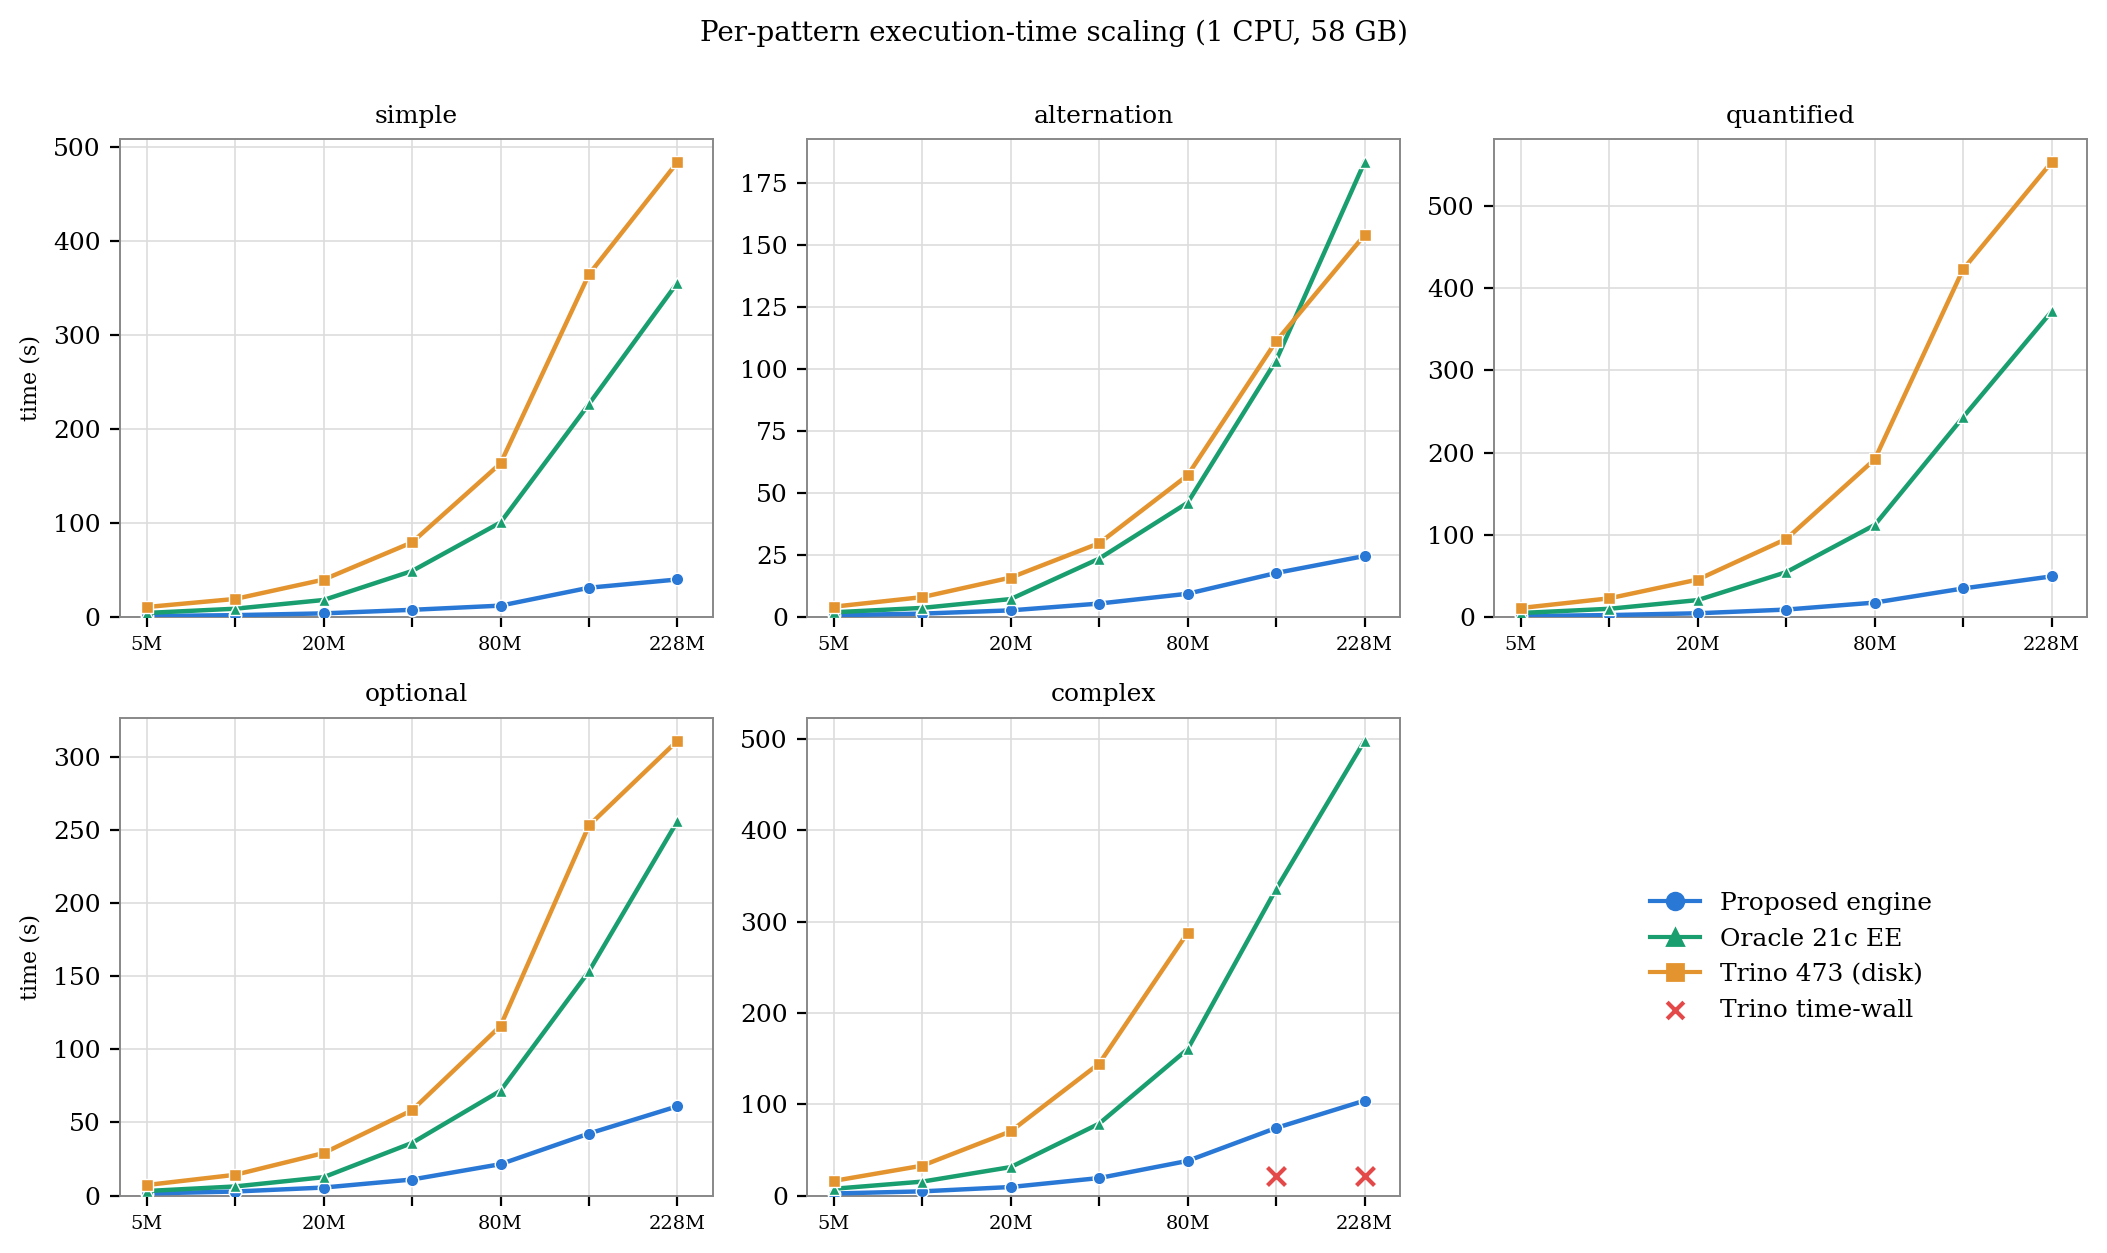
\includegraphics[width=\textwidth]{images/viz_stress_time_grid.png}
  \caption[Per-pattern execution-time scaling]{Per-pattern
    execution-time scaling on real data under a one-CPU and 58\,GB
    resource budget, with one panel per pattern family.  Completed runs
    remain close to linear over the evaluated sizes, although Oracle
    shows some super-linear drift.  The engine records the lowest
    execution time in every completed comparison.  Trino's
    \texttt{complex\_nested} runs reach the 600-second time limit at
    160~million and 227.9~million rows, shown by red $\times$ symbols.}
  \label{fig:stress_time_grid}
\end{figure}

\begin{table}[htbp]
\centering
\caption{Stress-test execution time (seconds, mean\,$\pm$\,std over five
  measured runs) for the three systems under identical conditions
  (1 CPU core, 58\,GB, real Amazon Reviews~2023 data, 5\,M--227.9\,M rows).
  \textit{wall} marks a query stopped at the 600\,s per-query time budget.
  Every completed database cell matched the engine's output row-for-row.}
\label{tab:stress_volume}
\resizebox{\textwidth}{!}{%
\begin{tabular}{@{}rccccc@{}}
\toprule
\textbf{Size (rows)} & \textbf{simple} & \textbf{altern.} & \textbf{quant.} & \textbf{optional} & \textbf{complex} \\
\midrule
\multicolumn{6}{@{}l}{\textit{Proposed engine}}\\*
5{,}000{,}000 & 0.6\,$\pm$\,0.0 & 0.7\,$\pm$\,0.0 & 0.6\,$\pm$\,0.0 & 0.6\,$\pm$\,0.0 & 2.2\,$\pm$\,0.0 \\
10{,}000{,}000 & 1.4\,$\pm$\,0.0 & 1.3\,$\pm$\,0.0 & 1.5\,$\pm$\,0.0 & 1.8\,$\pm$\,0.0 & 4.6\,$\pm$\,0.1 \\
20{,}000{,}000 & 3.0\,$\pm$\,0.0 & 2.6\,$\pm$\,0.0 & 3.1\,$\pm$\,0.0 & 3.6\,$\pm$\,0.0 & 9.3\,$\pm$\,0.1 \\
40{,}000{,}000 & 5.9\,$\pm$\,0.0 & 5.3\,$\pm$\,0.0 & 6.2\,$\pm$\,0.0 & 7.2\,$\pm$\,0.0 & 19.0\,$\pm$\,0.1 \\
80{,}000{,}000 & 10.5\,$\pm$\,0.6 & 9.1\,$\pm$\,0.0 & 11.1\,$\pm$\,0.4 & 13.3\,$\pm$\,0.6 & 36.9\,$\pm$\,0.6 \\
160{,}000{,}000 & 20.8\,$\pm$\,0.2 & 17.9\,$\pm$\,0.0 & 23.7\,$\pm$\,0.1 & 28.0\,$\pm$\,0.0 & 74.6\,$\pm$\,1.3 \\
227{,}899{,}533 & 30.9\,$\pm$\,0.1 & 24.7\,$\pm$\,0.0 & 33.5\,$\pm$\,0.1 & 40.1\,$\pm$\,0.0 & 102.6\,$\pm$\,2.8 \\
\addlinespace[3pt]
\multicolumn{6}{@{}l}{\textit{Oracle~21c EE}}\\*
5{,}000{,}000 & 4.3\,$\pm$\,0.0 & 1.9\,$\pm$\,0.0 & 4.8\,$\pm$\,0.0 & 3.1\,$\pm$\,0.0 & 7.4\,$\pm$\,0.0 \\
10{,}000{,}000 & 8.8\,$\pm$\,0.0 & 3.7\,$\pm$\,0.0 & 10.0\,$\pm$\,0.1 & 6.2\,$\pm$\,0.0 & 15.3\,$\pm$\,0.1 \\
20{,}000{,}000 & 18.1\,$\pm$\,0.1 & 7.2\,$\pm$\,0.0 & 20.5\,$\pm$\,0.0 & 12.6\,$\pm$\,0.1 & 31.2\,$\pm$\,0.1 \\
40{,}000{,}000 & 48.9\,$\pm$\,0.4 & 23.5\,$\pm$\,0.6 & 54.5\,$\pm$\,0.7 & 36.0\,$\pm$\,0.4 & 78.8\,$\pm$\,0.7 \\
80{,}000{,}000 & 100.6\,$\pm$\,1.2 & 46.1\,$\pm$\,1.3 & 112.0\,$\pm$\,1.2 & 71.7\,$\pm$\,1.1 & 160.3\,$\pm$\,1.4 \\
160{,}000{,}000 & 226.6\,$\pm$\,2.0 & 103.4\,$\pm$\,3.8 & 243.3\,$\pm$\,4.4 & 153.3\,$\pm$\,3.4 & 335.5\,$\pm$\,4.4 \\
227{,}899{,}533 & 355.6\,$\pm$\,8.9 & 183.5\,$\pm$\,9.1 & 371.8\,$\pm$\,8.0 & 255.9\,$\pm$\,7.6 & 498.0\,$\pm$\,9.5 \\
\addlinespace[3pt]
\multicolumn{6}{@{}l}{\textit{Trino~473 (disk connector)}}\\*
5{,}000{,}000 & 10.6\,$\pm$\,0.2 & 4.2\,$\pm$\,0.2 & 10.9\,$\pm$\,0.3 & 7.2\,$\pm$\,0.1 & 16.0\,$\pm$\,0.0 \\
10{,}000{,}000 & 19.2\,$\pm$\,0.2 & 8.0\,$\pm$\,0.1 & 22.7\,$\pm$\,0.5 & 14.2\,$\pm$\,0.1 & 32.7\,$\pm$\,0.3 \\
20{,}000{,}000 & 39.7\,$\pm$\,0.4 & 15.9\,$\pm$\,0.1 & 45.5\,$\pm$\,0.1 & 29.0\,$\pm$\,0.1 & 70.3\,$\pm$\,0.1 \\
40{,}000{,}000 & 79.3\,$\pm$\,0.5 & 29.8\,$\pm$\,0.1 & 95.0\,$\pm$\,0.5 & 58.3\,$\pm$\,0.2 & 144.5\,$\pm$\,2.8 \\
80{,}000{,}000 & 163.4\,$\pm$\,0.9 & 57.1\,$\pm$\,0.1 & 191.8\,$\pm$\,0.4 & 116.0\,$\pm$\,0.2 & 287.8\,$\pm$\,0.5 \\
160{,}000{,}000 & 364.6\,$\pm$\,2.0 & 111.2\,$\pm$\,0.7 & 423.3\,$\pm$\,1.0 & 253.0\,$\pm$\,6.5 & \textit{wall} \\
227{,}899{,}533 & 483.8\,$\pm$\,17.3 & 154.0\,$\pm$\,0.9 & 553.6\,$\pm$\,2.8 & 310.9\,$\pm$\,1.6 & \textit{wall} \\
\addlinespace[3pt]
\bottomrule
\end{tabular}}
\end{table}

\begin{table}[htbp]
\centering
\caption{Stress-test peak resident memory (GB, cgroup~v2 absolute peak
  during the query) for the three systems, same run as
  Table~\ref{tab:stress_volume}.  The engine holds data in RAM (rising to
  35.9\,GB on the heaviest family at 227.9\,M rows); Oracle~EE and Trino
  stream from disk behind a fixed working-memory floor.  \textit{wall} is
  as in Table~\ref{tab:stress_volume}.}
\label{tab:stress_mem}
\resizebox{\textwidth}{!}{%
\begin{tabular}{@{}rccccc@{}}
\toprule
\textbf{Size (rows)} & \textbf{simple} & \textbf{altern.} & \textbf{quant.} & \textbf{optional} & \textbf{complex} \\
\midrule
\multicolumn{6}{@{}l}{\textit{Proposed engine}}\\*
5{,}000{,}000 & 0.66 & 0.57 & 0.72 & 0.78 & 0.75 \\
10{,}000{,}000 & 1.3 & 1.3 & 1.4 & 1.5 & 1.5 \\
20{,}000{,}000 & 2.6 & 2.5 & 2.9 & 3.1 & 3.1 \\
40{,}000{,}000 & 5.0 & 4.8 & 5.6 & 6.0 & 6.0 \\
80{,}000{,}000 & 9.5 & 9.0 & 10.8 & 11.6 & 9.9 \\
160{,}000{,}000 & 18.7 & 17.5 & 21.1 & 22.7 & 19.3 \\
227{,}899{,}533 & 30.3 & 28.6 & 33.7 & 35.9 & 31.1 \\
\addlinespace[3pt]
\multicolumn{6}{@{}l}{\textit{Oracle~21c EE}}\\*
5{,}000{,}000 & 15.5 & 15.5 & 15.5 & 15.5 & 15.5 \\
10{,}000{,}000 & 15.2 & 15.3 & 15.3 & 15.3 & 15.3 \\
20{,}000{,}000 & 15.7 & 15.7 & 15.8 & 15.7 & 15.9 \\
40{,}000{,}000 & 17.2 & 17.2 & 17.4 & 17.4 & 17.4 \\
80{,}000{,}000 & 19.8 & 19.9 & 20.0 & 19.9 & 20.0 \\
160{,}000{,}000 & 25.6 & 25.6 & 25.6 & 25.7 & 25.7 \\
227{,}899{,}533 & 27.0 & 26.9 & 27.0 & 27.7 & 27.7 \\
\addlinespace[3pt]
\multicolumn{6}{@{}l}{\textit{Trino~473 (disk connector)}}\\*
5{,}000{,}000 & 13.3 & 13.4 & 13.4 & 13.4 & 13.4 \\
10{,}000{,}000 & 13.6 & 13.6 & 13.6 & 13.6 & 13.8 \\
20{,}000{,}000 & 13.9 & 13.9 & 13.9 & 14.1 & 16.2 \\
40{,}000{,}000 & 19.0 & 20.5 & 21.4 & 22.9 & 27.2 \\
80{,}000{,}000 & 25.3 & 30.1 & 38.4 & 47.5 & 47.5 \\
160{,}000{,}000 & 30.6 & 39.2 & 47.9 & 48.0 & \textit{wall} \\
227{,}899{,}533 & 37.8 & 47.5 & 47.5 & 36.4 & \textit{wall} \\
\addlinespace[3pt]
\bottomrule
\end{tabular}}
\end{table}

\begin{table}[htbp]
\centering
\caption{Stress-test throughput (million rows per second, size/mean-time) for the three systems, same run as Table~\ref{tab:stress_volume}.  Higher is better; the engine's size averages hold 6.6--8.1\,M\,rows/s over the four families every system completed, spanning 2.2\,M (\texttt{complex\_nested}) to 8.2\,M (\texttt{alternation}) per pattern.  \textit{wall} is as in Table~\ref{tab:stress_volume}.}
\label{tab:stress_thr}
\resizebox{\textwidth}{!}{%
\begin{tabular}{@{}rccccc@{}}
\toprule
\textbf{Size (rows)} & \textbf{simple} & \textbf{altern.} & \textbf{quant.} & \textbf{optional} & \textbf{complex} \\
\midrule
\multicolumn{6}{@{}l}{\textit{Proposed engine}}\\*
5{,}000{,}000 & 8.44 & 7.52 & 8.71 & 7.72 & 2.26 \\
10{,}000{,}000 & 6.96 & 7.52 & 6.58 & 5.51 & 2.16 \\
20{,}000{,}000 & 6.76 & 7.70 & 6.49 & 5.56 & 2.16 \\
40{,}000{,}000 & 6.82 & 7.59 & 6.46 & 5.53 & 2.11 \\
80{,}000{,}000 & 7.66 & 8.75 & 7.25 & 6.03 & 2.17 \\
160{,}000{,}000 & 7.70 & 8.95 & 6.75 & 5.72 & 2.14 \\
227{,}899{,}533 & 7.37 & 9.24 & 6.80 & 5.69 & 2.22 \\
\addlinespace[3pt]
\multicolumn{6}{@{}l}{\textit{Oracle~21c EE}}\\*
5{,}000{,}000 & 1.17 & 2.66 & 1.03 & 1.62 & 0.67 \\
10{,}000{,}000 & 1.14 & 2.74 & 1.00 & 1.61 & 0.66 \\
20{,}000{,}000 & 1.11 & 2.77 & 0.97 & 1.59 & 0.64 \\
40{,}000{,}000 & 0.82 & 1.70 & 0.73 & 1.11 & 0.51 \\
80{,}000{,}000 & 0.80 & 1.74 & 0.71 & 1.12 & 0.50 \\
160{,}000{,}000 & 0.71 & 1.55 & 0.66 & 1.04 & 0.48 \\
227{,}899{,}533 & 0.64 & 1.24 & 0.61 & 0.89 & 0.46 \\
\addlinespace[3pt]
\multicolumn{6}{@{}l}{\textit{Trino~473 (disk connector)}}\\*
5{,}000{,}000 & 0.47 & 1.21 & 0.46 & 0.69 & 0.31 \\
10{,}000{,}000 & 0.52 & 1.25 & 0.44 & 0.70 & 0.31 \\
20{,}000{,}000 & 0.50 & 1.26 & 0.44 & 0.69 & 0.28 \\
40{,}000{,}000 & 0.50 & 1.34 & 0.42 & 0.69 & 0.28 \\
80{,}000{,}000 & 0.49 & 1.40 & 0.42 & 0.69 & 0.28 \\
160{,}000{,}000 & 0.44 & 1.44 & 0.38 & 0.63 & \textit{wall} \\
227{,}899{,}533 & 0.46 & 1.48 & 0.41 & 0.73 & \textit{wall} \\
\addlinespace[3pt]
\bottomrule
\end{tabular}}
\end{table}

\begin{table}[htbp]
\centering
\caption{Stress-test incremental peak memory (GB): the cgroup~v2 absolute peak minus the five-second pre-query baseline---the per-query working memory on the same instrument for all three systems.  The engine holds the data it scans, so its incremental peak grows with $n$; the databases stream from disk and stay low (Trino's near-zero readings are the pre-committed-JVM-heap floor of Section~\ref{subsec:eval-memory}).  \textit{wall} is as in Table~\ref{tab:stress_volume}.}
\label{tab:stress_incmem}
\resizebox{\textwidth}{!}{%
\begin{tabular}{@{}rccccc@{}}
\toprule
\textbf{Size (rows)} & \textbf{simple} & \textbf{altern.} & \textbf{quant.} & \textbf{optional} & \textbf{complex} \\
\midrule
\multicolumn{6}{@{}l}{\textit{Proposed engine}}\\*
5{,}000{,}000 & 0.32 & 0.21 & 0.35 & 0.40 & 0.31 \\
10{,}000{,}000 & 0.59 & 0.51 & 0.70 & 0.79 & 0.63 \\
20{,}000{,}000 & 1.2 & 1.0 & 1.5 & 1.6 & 1.4 \\
40{,}000{,}000 & 2.4 & 2.0 & 2.9 & 3.2 & 2.7 \\
80{,}000{,}000 & 4.9 & 4.0 & 5.9 & 6.5 & 4.2 \\
160{,}000{,}000 & 9.8 & 8.0 & 11.8 & 12.9 & 8.4 \\
227{,}899{,}533 & 14.0 & 11.4 & 16.8 & 18.4 & 12.0 \\
\addlinespace[3pt]
\multicolumn{6}{@{}l}{\textit{Oracle~21c EE}}\\*
5{,}000{,}000 & 0.13 & 0.13 & 0.13 & 0.13 & 0.13 \\
10{,}000{,}000 & 0.26 & 0.26 & 0.26 & 0.26 & 0.26 \\
20{,}000{,}000 & 0.52 & 0.51 & 0.51 & 0.51 & 0.52 \\
40{,}000{,}000 & 0.45 & 0.45 & 0.45 & 0.45 & 0.45 \\
80{,}000{,}000 & 0.46 & 0.45 & 0.46 & 0.45 & 0.46 \\
160{,}000{,}000 & 0.47 & 0.46 & 0.46 & 0.47 & 0.49 \\
227{,}899{,}533 & 0.68 & 0.65 & 0.64 & 0.55 & 0.59 \\
\addlinespace[3pt]
\multicolumn{6}{@{}l}{\textit{Trino~473 (disk connector)}}\\*
5{,}000{,}000 & 0.007 & 0.003 & 0.004 & 0.002 & 0.004 \\
10{,}000{,}000 & 0.006 & 0.008 & 0.004 & 0.008 & 0.005 \\
20{,}000{,}000 & 0.006 & 0.006 & 0.006 & 0.004 & 0.36 \\
40{,}000{,}000 & 0.73 & 0.007 & 0.45 & 0.02 & 0.72 \\
80{,}000{,}000 & 1.5 & 0.02 & 1.5 & 0.01 & 0.01 \\
160{,}000{,}000 & 1.6 & 2.6 & 0.03 & 0.01 & \textit{wall} \\
227{,}899{,}533 & 2.7 & 1.4 & 0.78 & 1.5 & \textit{wall} \\
\addlinespace[3pt]
\bottomrule
\end{tabular}}
\end{table}

\begin{table}[htbp]
\centering
\caption{Databases' own per-query memory counters (GB): Oracle's session PGA high-water mark and Trino's reported \texttt{peakMemoryBytes}.  These confirm the small per-query working sets behind the fixed SGA/JVM baselines (the engine has no separate counter---it is the measured process).  \textit{wall} is as in Table~\ref{tab:stress_volume}.}
\label{tab:stress_native}
\resizebox{\textwidth}{!}{%
\begin{tabular}{@{}rccccc@{}}
\toprule
\textbf{Size (rows)} & \textbf{simple} & \textbf{altern.} & \textbf{quant.} & \textbf{optional} & \textbf{complex} \\
\midrule
\multicolumn{6}{@{}l}{\textit{Oracle~21c EE}}\\*
5{,}000{,}000 & 0.13 & 0.13 & 0.13 & 0.13 & 0.13 \\
10{,}000{,}000 & 0.26 & 0.26 & 0.26 & 0.26 & 0.26 \\
20{,}000{,}000 & 0.52 & 0.52 & 0.52 & 0.52 & 0.52 \\
40{,}000{,}000 & 0.45 & 0.45 & 0.45 & 0.45 & 0.45 \\
80{,}000{,}000 & 0.45 & 0.45 & 0.45 & 0.45 & 0.45 \\
160{,}000{,}000 & 0.45 & 0.45 & 0.45 & 0.46 & 0.46 \\
227{,}899{,}533 & 0.45 & 0.45 & 0.45 & 0.46 & 0.46 \\
\addlinespace[3pt]
\multicolumn{6}{@{}l}{\textit{Trino~473 (disk connector)}}\\*
5{,}000{,}000 & 0.09 & 0.09 & 0.09 & 0.09 & 0.09 \\
10{,}000{,}000 & 0.19 & 0.19 & 0.19 & 0.19 & 0.19 \\
20{,}000{,}000 & 0.33 & 0.33 & 0.33 & 0.33 & 0.33 \\
40{,}000{,}000 & 0.71 & 0.71 & 0.71 & 0.71 & 0.71 \\
80{,}000{,}000 & 1.5 & 1.5 & 1.5 & 1.5 & 1.5 \\
160{,}000{,}000 & 2.6 & 2.6 & 2.6 & 2.6 & \textit{wall} \\
227{,}899{,}533 & 3.8 & 3.8 & 3.8 & 3.8 & \textit{wall} \\
\addlinespace[3pt]
\bottomrule
\end{tabular}}
\end{table}

\begin{table}[htbp]
\centering
\caption{Match counts (\texttt{ONE ROW PER MATCH} output rows) per pattern and size.  All three systems returned identical counts and passed row-level equality against the engine at every completed cell, so a single column per cell suffices.}
\label{tab:stress_matches}
\resizebox{\textwidth}{!}{%
\begin{tabular}{@{}rccccc@{}}
\toprule
\textbf{Size (rows)} & \textbf{simple} & \textbf{altern.} & \textbf{quant.} & \textbf{optional} & \textbf{complex} \\
\midrule
5{,}000{,}000 & 591{,}476 & 103{,}496 & 323{,}805 & 309{,}050 & 351{,}661 \\
10{,}000{,}000 & 1{,}150{,}566 & 193{,}114 & 631{,}723 & 605{,}909 & 681{,}288 \\
20{,}000{,}000 & 2{,}289{,}658 & 369{,}406 & 1{,}272{,}734 & 1{,}224{,}714 & 1{,}361{,}317 \\
40{,}000{,}000 & 4{,}399{,}482 & 665{,}442 & 2{,}470{,}577 & 2{,}389{,}804 & 2{,}617{,}208 \\
80{,}000{,}000 & 8{,}216{,}302 & 1{,}190{,}587 & 4{,}727{,}306 & 4{,}597{,}581 & 4{,}974{,}189 \\
160{,}000{,}000 & 14{,}293{,}355 & 1{,}960{,}129 & 8{,}716{,}637 & 8{,}536{,}256 & 9{,}102{,}417 \\
227{,}899{,}533 & 18{,}836{,}350 & 2{,}656{,}560 & 12{,}355{,}865 & 12{,}134{,}528 & 12{,}900{,}322 \\
\bottomrule
\end{tabular}}
\end{table}
